\documentclass{standalone}
\usepackage{tikz}
\usetikzlibrary{patterns, positioning}


\begin{document}
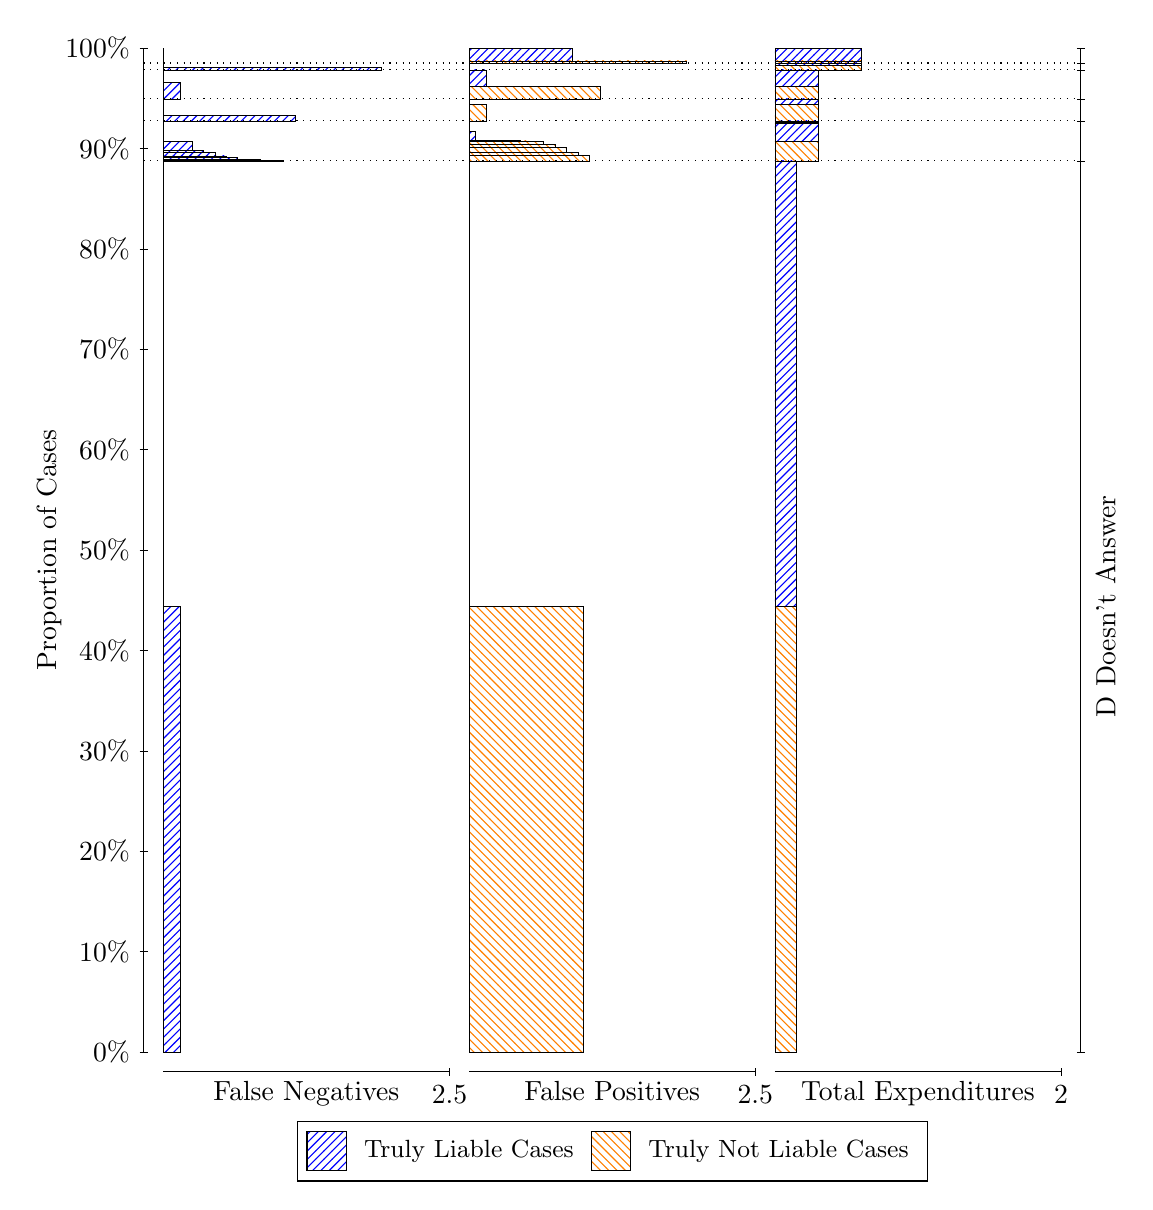
\begin{tikzpicture}
\draw[black, very thin] (1.5,1.75) -- (1.5,14.5);
\node[rotate=90, text=black, anchor=center] at (0.3, 8.125) {Proportion of Cases};
\draw[black, very thin] (1.45,1.75) -- (1.55,1.75);
\node[text=black, anchor=east] at (1.45, 1.75) {0\%};
\draw[black, very thin] (1.45,3.025) -- (1.55,3.025);
\node[text=black, anchor=east] at (1.45, 3.025) {10\%};
\draw[black, very thin] (1.45,4.3) -- (1.55,4.3);
\node[text=black, anchor=east] at (1.45, 4.3) {20\%};
\draw[black, very thin] (1.45,5.575) -- (1.55,5.575);
\node[text=black, anchor=east] at (1.45, 5.575) {30\%};
\draw[black, very thin] (1.45,6.85) -- (1.55,6.85);
\node[text=black, anchor=east] at (1.45, 6.85) {40\%};
\draw[black, very thin] (1.45,8.125) -- (1.55,8.125);
\node[text=black, anchor=east] at (1.45, 8.125) {50\%};
\draw[black, very thin] (1.45,9.4) -- (1.55,9.4);
\node[text=black, anchor=east] at (1.45, 9.4) {60\%};
\draw[black, very thin] (1.45,10.675) -- (1.55,10.675);
\node[text=black, anchor=east] at (1.45, 10.675) {70\%};
\draw[black, very thin] (1.45,11.95) -- (1.55,11.95);
\node[text=black, anchor=east] at (1.45, 11.95) {80\%};
\draw[black, very thin] (1.45,13.225) -- (1.55,13.225);
\node[text=black, anchor=east] at (1.45, 13.225) {90\%};
\draw[black, very thin] (1.45,14.5) -- (1.55,14.5);
\node[text=black, anchor=east] at (1.45, 14.5) {100\%};

\draw[black, very thin] (13.4,1.75) -- (13.4,14.5);
\draw[black, very thin] (13.35,1.75) -- (13.45,1.75);
\node[anchor=west] at (13.35, 1.75) {};
\draw[black, very thin] (13.35,13.067) -- (13.45,13.067);
\node[anchor=west] at (13.35, 13.067) {};
\draw[black, very thin] (13.35,13.575) -- (13.45,13.575);
\node[anchor=west] at (13.35, 13.575) {};
\draw[black, very thin] (13.35,13.855) -- (13.45,13.855);
\node[anchor=west] at (13.35, 13.855) {};
\draw[black, very thin] (13.35,14.223) -- (13.45,14.223);
\node[anchor=west] at (13.35, 14.223) {};
\draw[black, very thin] (13.35,14.31) -- (13.45,14.31);
\node[anchor=west] at (13.35, 14.31) {};
\draw[black, very thin] (13.35,14.5) -- (13.45,14.5);
\node[anchor=west] at (13.35, 14.5) {};

\draw[black, very thin, pattern color=blue, pattern=north east lines] (1.75,1.75) rectangle (1.968,7.4085);
\draw[black, very thin, pattern color=orange, pattern=north west lines] (1.75,7.4085) rectangle (1.75,13.067);
\draw[black, very thin, pattern color=blue, pattern=north east lines] (1.75,13.067) rectangle (3.276,13.071);
\draw[black, very thin, pattern color=blue, pattern=north east lines] (1.75,13.071) rectangle (3.1307,13.074);
\draw[black, very thin, pattern color=blue, pattern=north east lines] (1.75,13.074) rectangle (2.9853,13.081);
\draw[black, very thin, pattern color=blue, pattern=north east lines] (1.75,13.081) rectangle (2.84,13.089);
\draw[black, very thin, pattern color=blue, pattern=north east lines] (1.75,13.089) rectangle (2.6947,13.111);
\draw[black, very thin, pattern color=blue, pattern=north east lines] (1.75,13.111) rectangle (2.5493,13.131);
\draw[black, very thin, pattern color=blue, pattern=north east lines] (1.75,13.131) rectangle (2.404,13.173);
\draw[black, very thin, pattern color=blue, pattern=north east lines] (1.75,13.173) rectangle (2.2587,13.2);
\draw[black, very thin, pattern color=blue, pattern=north east lines] (1.75,13.2) rectangle (2.1133,13.311);
\draw[black, very thin, pattern color=orange, pattern=north west lines] (1.75,13.311) rectangle (1.75,13.575);
\draw[black, very thin, pattern color=blue, pattern=north east lines] (1.75,13.575) rectangle (3.4213,13.648);
\draw[black, very thin, pattern color=orange, pattern=north west lines] (1.75,13.648) rectangle (1.75,13.855);
\draw[black, very thin, pattern color=blue, pattern=north east lines] (1.75,13.855) rectangle (1.968,14.065);
\draw[black, very thin, pattern color=orange, pattern=north west lines] (1.75,14.065) rectangle (1.75,14.223);
\draw[black, very thin, pattern color=blue, pattern=north east lines] (1.75,14.223) rectangle (4.5113,14.251);
\draw[black, very thin, pattern color=orange, pattern=north west lines] (1.75,14.251) rectangle (1.75,14.31);
\draw[black, very thin, pattern color=orange, pattern=north west lines] (1.75,14.31) rectangle (1.75,14.338);
\draw[black, very thin, pattern color=blue, pattern=north east lines] (1.75,14.338) rectangle (1.75,14.5);
\draw[black, very thin, pattern color=orange, pattern=north west lines] (5.6333,1.75) rectangle (7.0867,7.4087);
\draw[black, very thin, pattern color=blue, pattern=north east lines] (5.6333,7.4087) rectangle (5.6333,13.067);
\draw[black, very thin, pattern color=orange, pattern=north west lines] (5.6333,13.067) rectangle (7.1593,13.136);
\draw[black, very thin, pattern color=orange, pattern=north west lines] (5.6333,13.136) rectangle (7.014,13.172);
\draw[black, very thin, pattern color=orange, pattern=north west lines] (5.6333,13.172) rectangle (6.8687,13.241);
\draw[black, very thin, pattern color=orange, pattern=north west lines] (5.6333,13.241) rectangle (6.7233,13.278);
\draw[black, very thin, pattern color=orange, pattern=north west lines] (5.6333,13.278) rectangle (6.578,13.313);
\draw[black, very thin, pattern color=orange, pattern=north west lines] (5.6333,13.313) rectangle (6.4327,13.316);
\draw[black, very thin, pattern color=orange, pattern=north west lines] (5.6333,13.316) rectangle (6.4327,13.32);
\draw[black, very thin, pattern color=orange, pattern=north west lines] (5.6333,13.32) rectangle (6.2873,13.326);
\draw[black, very thin, pattern color=orange, pattern=north west lines] (5.6333,13.326) rectangle (6.142,13.328);
\draw[black, very thin, pattern color=orange, pattern=north west lines] (5.6333,13.328) rectangle (5.9967,13.331);
\draw[black, very thin, pattern color=blue, pattern=north east lines] (5.6333,13.331) rectangle (5.706,13.442);
\draw[black, very thin, pattern color=blue, pattern=north east lines] (5.6333,13.442) rectangle (5.6333,13.575);
\draw[black, very thin, pattern color=orange, pattern=north west lines] (5.6333,13.575) rectangle (5.8513,13.782);
\draw[black, very thin, pattern color=blue, pattern=north east lines] (5.6333,13.782) rectangle (5.6333,13.855);
\draw[black, very thin, pattern color=orange, pattern=north west lines] (5.6333,13.855) rectangle (7.3047,14.013);
\draw[black, very thin, pattern color=blue, pattern=north east lines] (5.6333,14.013) rectangle (5.8513,14.223);
\draw[black, very thin, pattern color=orange, pattern=north west lines] (5.6333,14.223) rectangle (5.6333,14.282);
\draw[black, very thin, pattern color=blue, pattern=north east lines] (5.6333,14.282) rectangle (5.6333,14.31);
\draw[black, very thin, pattern color=orange, pattern=north west lines] (5.6333,14.31) rectangle (8.3947,14.338);
\draw[black, very thin, pattern color=blue, pattern=north east lines] (5.6333,14.338) rectangle (6.9413,14.5);
\draw[black, very thin, pattern color=orange, pattern=north west lines] (9.5167,1.75) rectangle (9.7892,7.4087);
\draw[black, very thin, pattern color=blue, pattern=north east lines] (9.5167,7.4087) rectangle (9.7892,13.067);
\draw[black, very thin, pattern color=orange, pattern=north west lines] (9.5167,13.067) rectangle (10.062,13.316);
\draw[black, very thin, pattern color=blue, pattern=north east lines] (9.5167,13.316) rectangle (10.062,13.541);
\draw[black, very thin, pattern color=orange, pattern=north west lines] (9.5167,13.541) rectangle (10.062,13.545);
\draw[black, very thin, pattern color=blue, pattern=north east lines] (9.5167,13.545) rectangle (10.062,13.548);
\draw[black, very thin, pattern color=orange, pattern=north west lines] (9.5167,13.548) rectangle (10.062,13.56);
\draw[black, very thin, pattern color=blue, pattern=north east lines] (9.5167,13.56) rectangle (10.062,13.575);
\draw[black, very thin, pattern color=orange, pattern=north west lines] (9.5167,13.575) rectangle (10.062,13.782);
\draw[black, very thin, pattern color=blue, pattern=north east lines] (9.5167,13.782) rectangle (10.062,13.855);
\draw[black, very thin, pattern color=orange, pattern=north west lines] (9.5167,13.855) rectangle (10.062,14.013);
\draw[black, very thin, pattern color=blue, pattern=north east lines] (9.5167,14.013) rectangle (10.062,14.223);
\draw[black, very thin, pattern color=orange, pattern=north west lines] (9.5167,14.223) rectangle (10.607,14.282);
\draw[black, very thin, pattern color=blue, pattern=north east lines] (9.5167,14.282) rectangle (10.607,14.31);
\draw[black, very thin, pattern color=orange, pattern=north west lines] (9.5167,14.31) rectangle (10.607,14.338);
\draw[black, very thin, pattern color=blue, pattern=north east lines] (9.5167,14.338) rectangle (10.607,14.5);
\draw[black, dotted] (1.5,13.067) -- (13.4,13.067);
\draw[black, dotted] (1.5,13.575) -- (13.4,13.575);
\draw[black, dotted] (1.5,13.855) -- (13.4,13.855);
\draw[black, dotted] (1.5,14.223) -- (13.4,14.223);
\draw[black, dotted] (1.5,14.31) -- (13.4,14.31);
\draw[black, very thin] (1.75,1.5) -- (5.3833,1.5);
\node[text=black, anchor=north] at (3.5667, 1.5) {False Negatives};
\draw[black, very thin] (5.3833,1.45) -- (5.3833,1.55);
\node[text=black, anchor=north] at (5.3833, 1.45) {2.5};

\draw[black, very thin] (5.6333,1.5) -- (9.2667,1.5);
\node[text=black, anchor=north] at (7.45, 1.5) {False Positives};
\draw[black, very thin] (9.2667,1.45) -- (9.2667,1.55);
\node[text=black, anchor=north] at (9.2667, 1.45) {2.5};

\draw[black, very thin] (9.5167,1.5) -- (13.15,1.5);
\node[text=black, anchor=north] at (11.333, 1.5) {Total Expenditures};
\draw[black, very thin] (13.15,1.45) -- (13.15,1.55);
\node[text=black, anchor=north] at (13.15, 1.45) {2};

\node[text=black, centered, rotate=90] at (13.72, 7.4086) {D Doesn't Answer};






\draw (7.449999999999999,1.5) node[draw=none] (baseCoordinate) {};
\begin{scope}[align=center]
        \matrix[scale=0.5, draw=black, below=0.5cm of baseCoordinate, nodes={draw}, column sep=0.1cm]{
            \node[rectangle, draw, minimum width=0.5cm, minimum height=0.5cm, pattern color=blue, pattern=north east lines] {}; &
            \node[draw=none, font=\small, text=black] (B) {Truly Liable Cases}; &
            \node[rectangle, draw, minimum width=0.5cm, minimum height=0.5cm, pattern color=orange, pattern=north west lines] {}; &
            \node[draw=none, font=\small, text=black] (B) {Truly Not Liable Cases}; \\
            };
\end{scope}

\end{tikzpicture}
\end{document}